\documentclass{article}

\usepackage{fancyhdr}
\usepackage{ragged2e}
\usepackage[table]{xcolor}
\usepackage{indentfirst}
\usepackage{longtable}
\usepackage{graphicx}
\usepackage{float}

\graphicspath{ {./imgs/} }

\makeatletter
\title{Documento de Arquitectura del Software} \let\Title\@title
\date{Septiembre 2018} \let\Date\@date
\author{Ricardo Münch} \let\Author\@author
\makeatother

\pagestyle{fancy}
\fancyhf{}
\rhead{Versión: 1.0 \\ \Date}
\lhead{eFuel \\ DAS \\ Identificador del documento}

\lfoot{Confidencial}
\cfoot{iKels Consulting \\ \Date}
\rfoot{Pag. \thepage}

\renewcommand{\headrulewidth}{1pt}
\renewcommand{\footrulewidth}{1pt}
\renewcommand{\contentsname}{Índice}

\begin{document}

    \begin{titlepage}
    \huge{\Title}
    \begin{flushright}
        \Large{eFuel \\ Versión: 1.0}
    \end{flushright}
    \end{titlepage}

    \newpage
    \tableofcontents

    \newpage
    \begin{center}
        \begin{tabular}{ |c|c|c|c| }
            \hline
            \rowcolor{lightgray}
            Fecha & Versión & Descripción & Autores \\
            \hline
            29/09/2018 & 1.0 & Documento de Arquitectura & Ricardo Münch \\
            \hline
        \end{tabular}
    \end{center}

    \newpage
    \section{Introducción}
    El objetivo principal de la arquitectura del software es aportar conceptos y un lenguaje común que ayuden a describir el software y permita la comunicación entre el cliente y los diseñadores.

    \subsection{Propósito}
    Este documento busca hacer una abstracción de lo que será el sistema a través de algunas vistas de la arquitectura del mismo. Se pretende definir algunos elementos estructurales que describen el sistema \emph{eFuel}.

    \subsection{Alcance}
    A continuación presentamos una abstracción de la estructura que debe tener el sistema. El documento contempla la vista lógica, la vista de datos y las características no funcionales que debe tener el sistema.

    \subsection{Referencias}
    No hace referencia a ningún otro documento.

    \subsection{Vista Global}
    Este documento comprende 6 secciones en las cuales se elaboran los distintos aspectos de la arquitectura de \emph{eFuel}, tanto a nivel de software como de hardware. En la sección \ref{reprArq} se introduce la representación arquitectónica del sistema. Luego, en la sección \ref{metasArq}, se enumeran los objetivos y restricciones que suscriben la arquitectura presentada. Seguidamente, se describen las distintas vistas que conforman la arquitectura de la sección \ref{vistaCasosDeUso} a la \ref{vistaDatos}, teniendo en la sección \ref{vistaCasosDeUso} la Vista de Casos de Uso. Finalmente, la sección \ref{tamDesemp}.


    \section{Representación Arquitectónica} \label{reprArq}
    La representación arquitectónica de \emph{eFuel} está basada en el modelo de 4+1 vistas de Philippe Kruchten. En el transcurso del documento se tratarán más a fondo los detalles de cada una.

    \section{Metas y Restricciones Arquitectónicas} \label{metasArq}


    \section{Vista de Casos de Uso} \label{vistaCasosDeUso}
    En esta vista se describirá el sistema desde el punto de vista de los casos de uso. El sistema tiene 2 actores:

    \begin{itemize}
        \item \emph{Customer}: distribuidor de combustible, puede tener una o varias estaciones de servicio a su cargo. Son los usuarios más frecuentes del sistema.
        \item \emph{Staff}: administrador del sistema. Tienen acceso al \emph{beack end} de Umbraco y pueden gestionar todas las entidades del sistema.
    \end{itemize}

    \subsection{Resumen de Casos de Uso}
    \newcounter{magicrownumbers}
    \newcommand\rownumber{\stepcounter{magicrownumbers}\arabic{magicrownumbers}}
    \begin{center}
        \begin{longtable}{ |c|c|c| }
            \hline

            \rowcolor{lightgray}
            ID Caso de Uso & Caso de Uso & Actor \\
            \endhead

            \hline
            \endfoot

            \hline
            CU-\rownumber & Gestionar cliente & Staff \\
            CU-\rownumber & Crear cliente & Staff \\
            CU-\rownumber & Consultar cliente & Staff, Customer \\
            CU-\rownumber & Editar cliente & Staff \\
            CU-\rownumber & Eliminar cliente/s & Staff \\
            CU-\rownumber & Consultar lista de clientes & Staff, Customer \\
            CU-\rownumber & Importar lista de clientes & Staff \\
            CU-\rownumber & Exportar lista de clientes & Staff, Customer \\

            CU-\rownumber & Gestionar transporte & Staff \\
            CU-\rownumber & Crear transporte & Staff \\
            CU-\rownumber & Consultar transporte & Staff, Customer \\
            CU-\rownumber & Editar transporte & Staff \\
            CU-\rownumber & Eliminar transporte/s & Staff \\
            CU-\rownumber & Consultar lista de transportes & Staff, Customer \\
            CU-\rownumber & Importar lista de transportes & Staff \\
            CU-\rownumber & Exportar lista de transportes & Staff, Customer \\

            CU-\rownumber & Gestionar zona & Staff \\
            CU-\rownumber & Crear zona & Staff \\
            CU-\rownumber & Consultar zona & Staff, Customer \\
            CU-\rownumber & Editar zona & Staff \\
            CU-\rownumber & Eliminar zona/s & Staff \\
            CU-\rownumber & Consultar lista de zonas & Staff, Customer \\
            CU-\rownumber & Importar lista de zonas & Staff \\
            CU-\rownumber & Exportar lista de zonas & Staff, Customer \\

            CU-\rownumber & Gestionar turno & Staff \\
            CU-\rownumber & Crear turno & Staff \\
            CU-\rownumber & Consultar turno & Staff \\
            CU-\rownumber & Editar turno & Staff \\
            CU-\rownumber & Eliminar turno/s & Staff \\
            CU-\rownumber & Consultar lista de turnos & Staff \\

            CU-\rownumber & Gestionar factura & Staff \\
            CU-\rownumber & Crear factura & Staff \\
            CU-\rownumber & Consultar factura & Staff, Customer \\
            CU-\rownumber & Editar factura & Staff \\
            CU-\rownumber & Eliminar factura/s & Staff \\
            CU-\rownumber & Consultar lista de facturas & Staff, Customer \\

            CU-\rownumber & Gestionar cobro & Staff \\
            CU-\rownumber & Crear cobro & Staff \\
            CU-\rownumber & Consultar cobro & Staff \\
            CU-\rownumber & Editar cobro & Staff \\
            CU-\rownumber & Eliminar cobro/s & Staff \\
            CU-\rownumber & Consultar lista de cobros & Staff \\
        \end{longtable}
    \end{center}

    \subsection{Diagrama de Casos de Uso}
    Se separaron los casos de uso en varios diagramas para facilitar la lectura.

    \begin{figure}[H]
        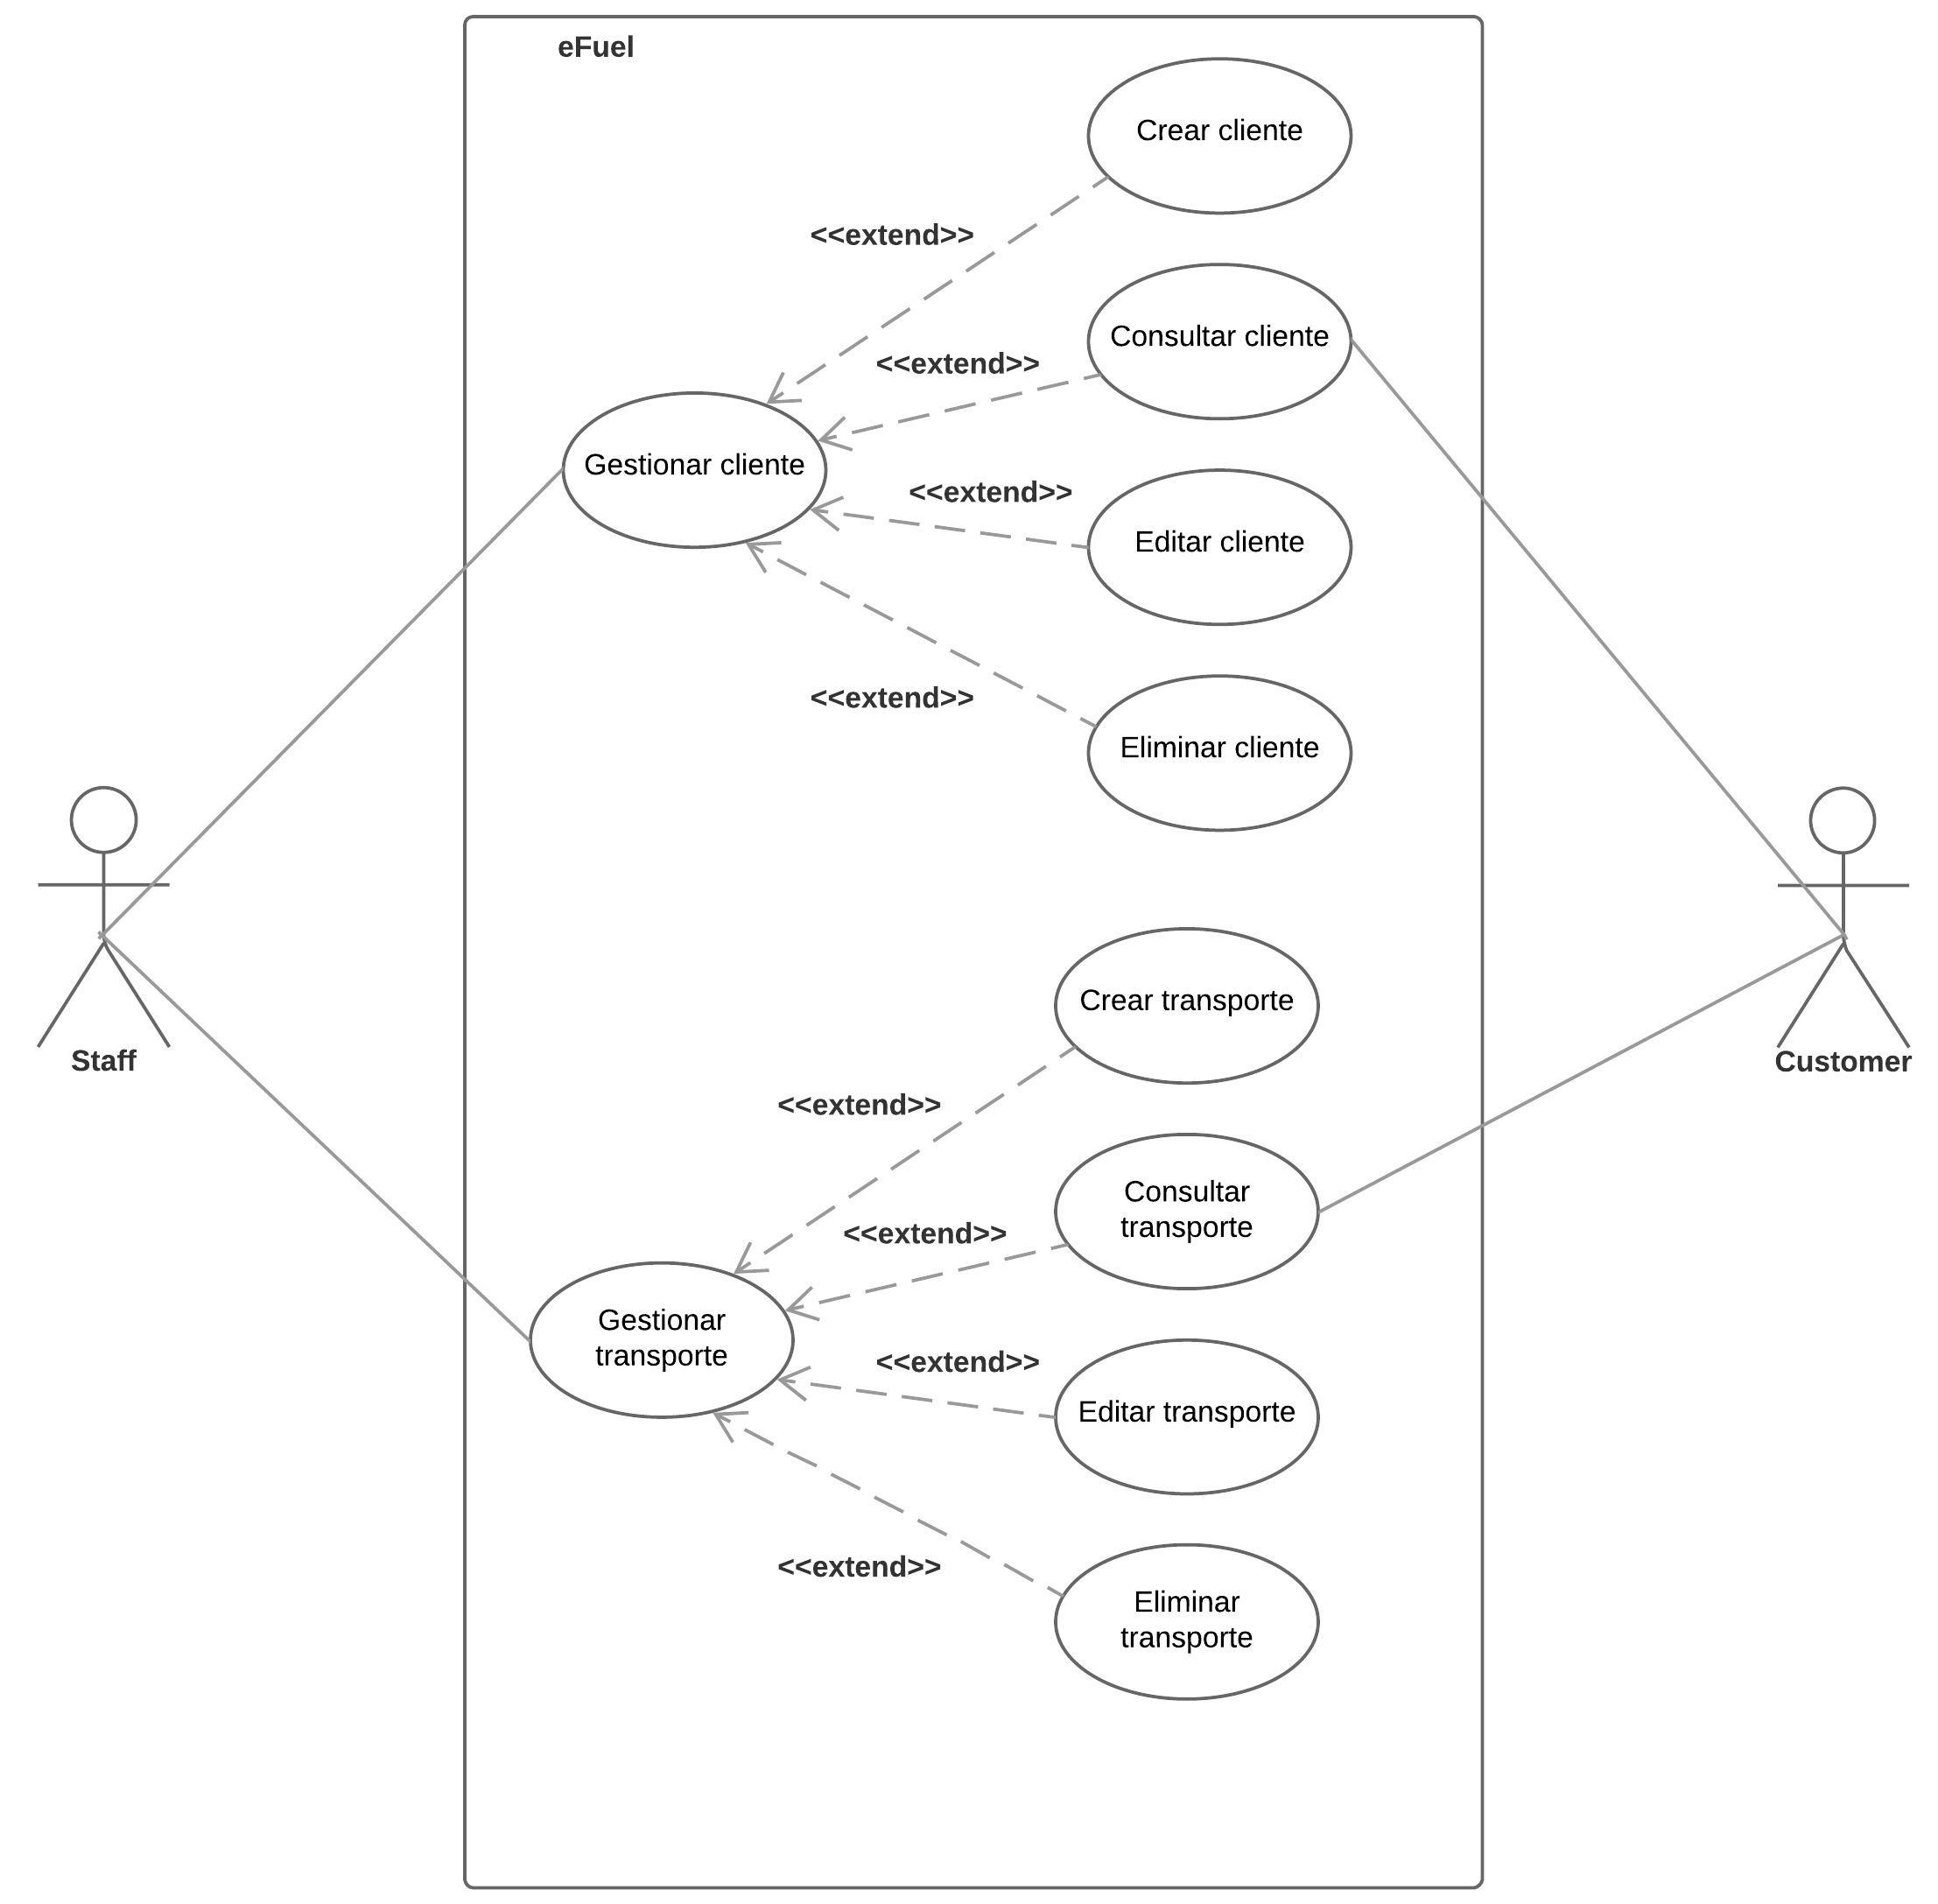
\includegraphics[width=\textwidth]{cu1.jpeg}
        \centering
    \end{figure}

    \begin{figure}[H]
        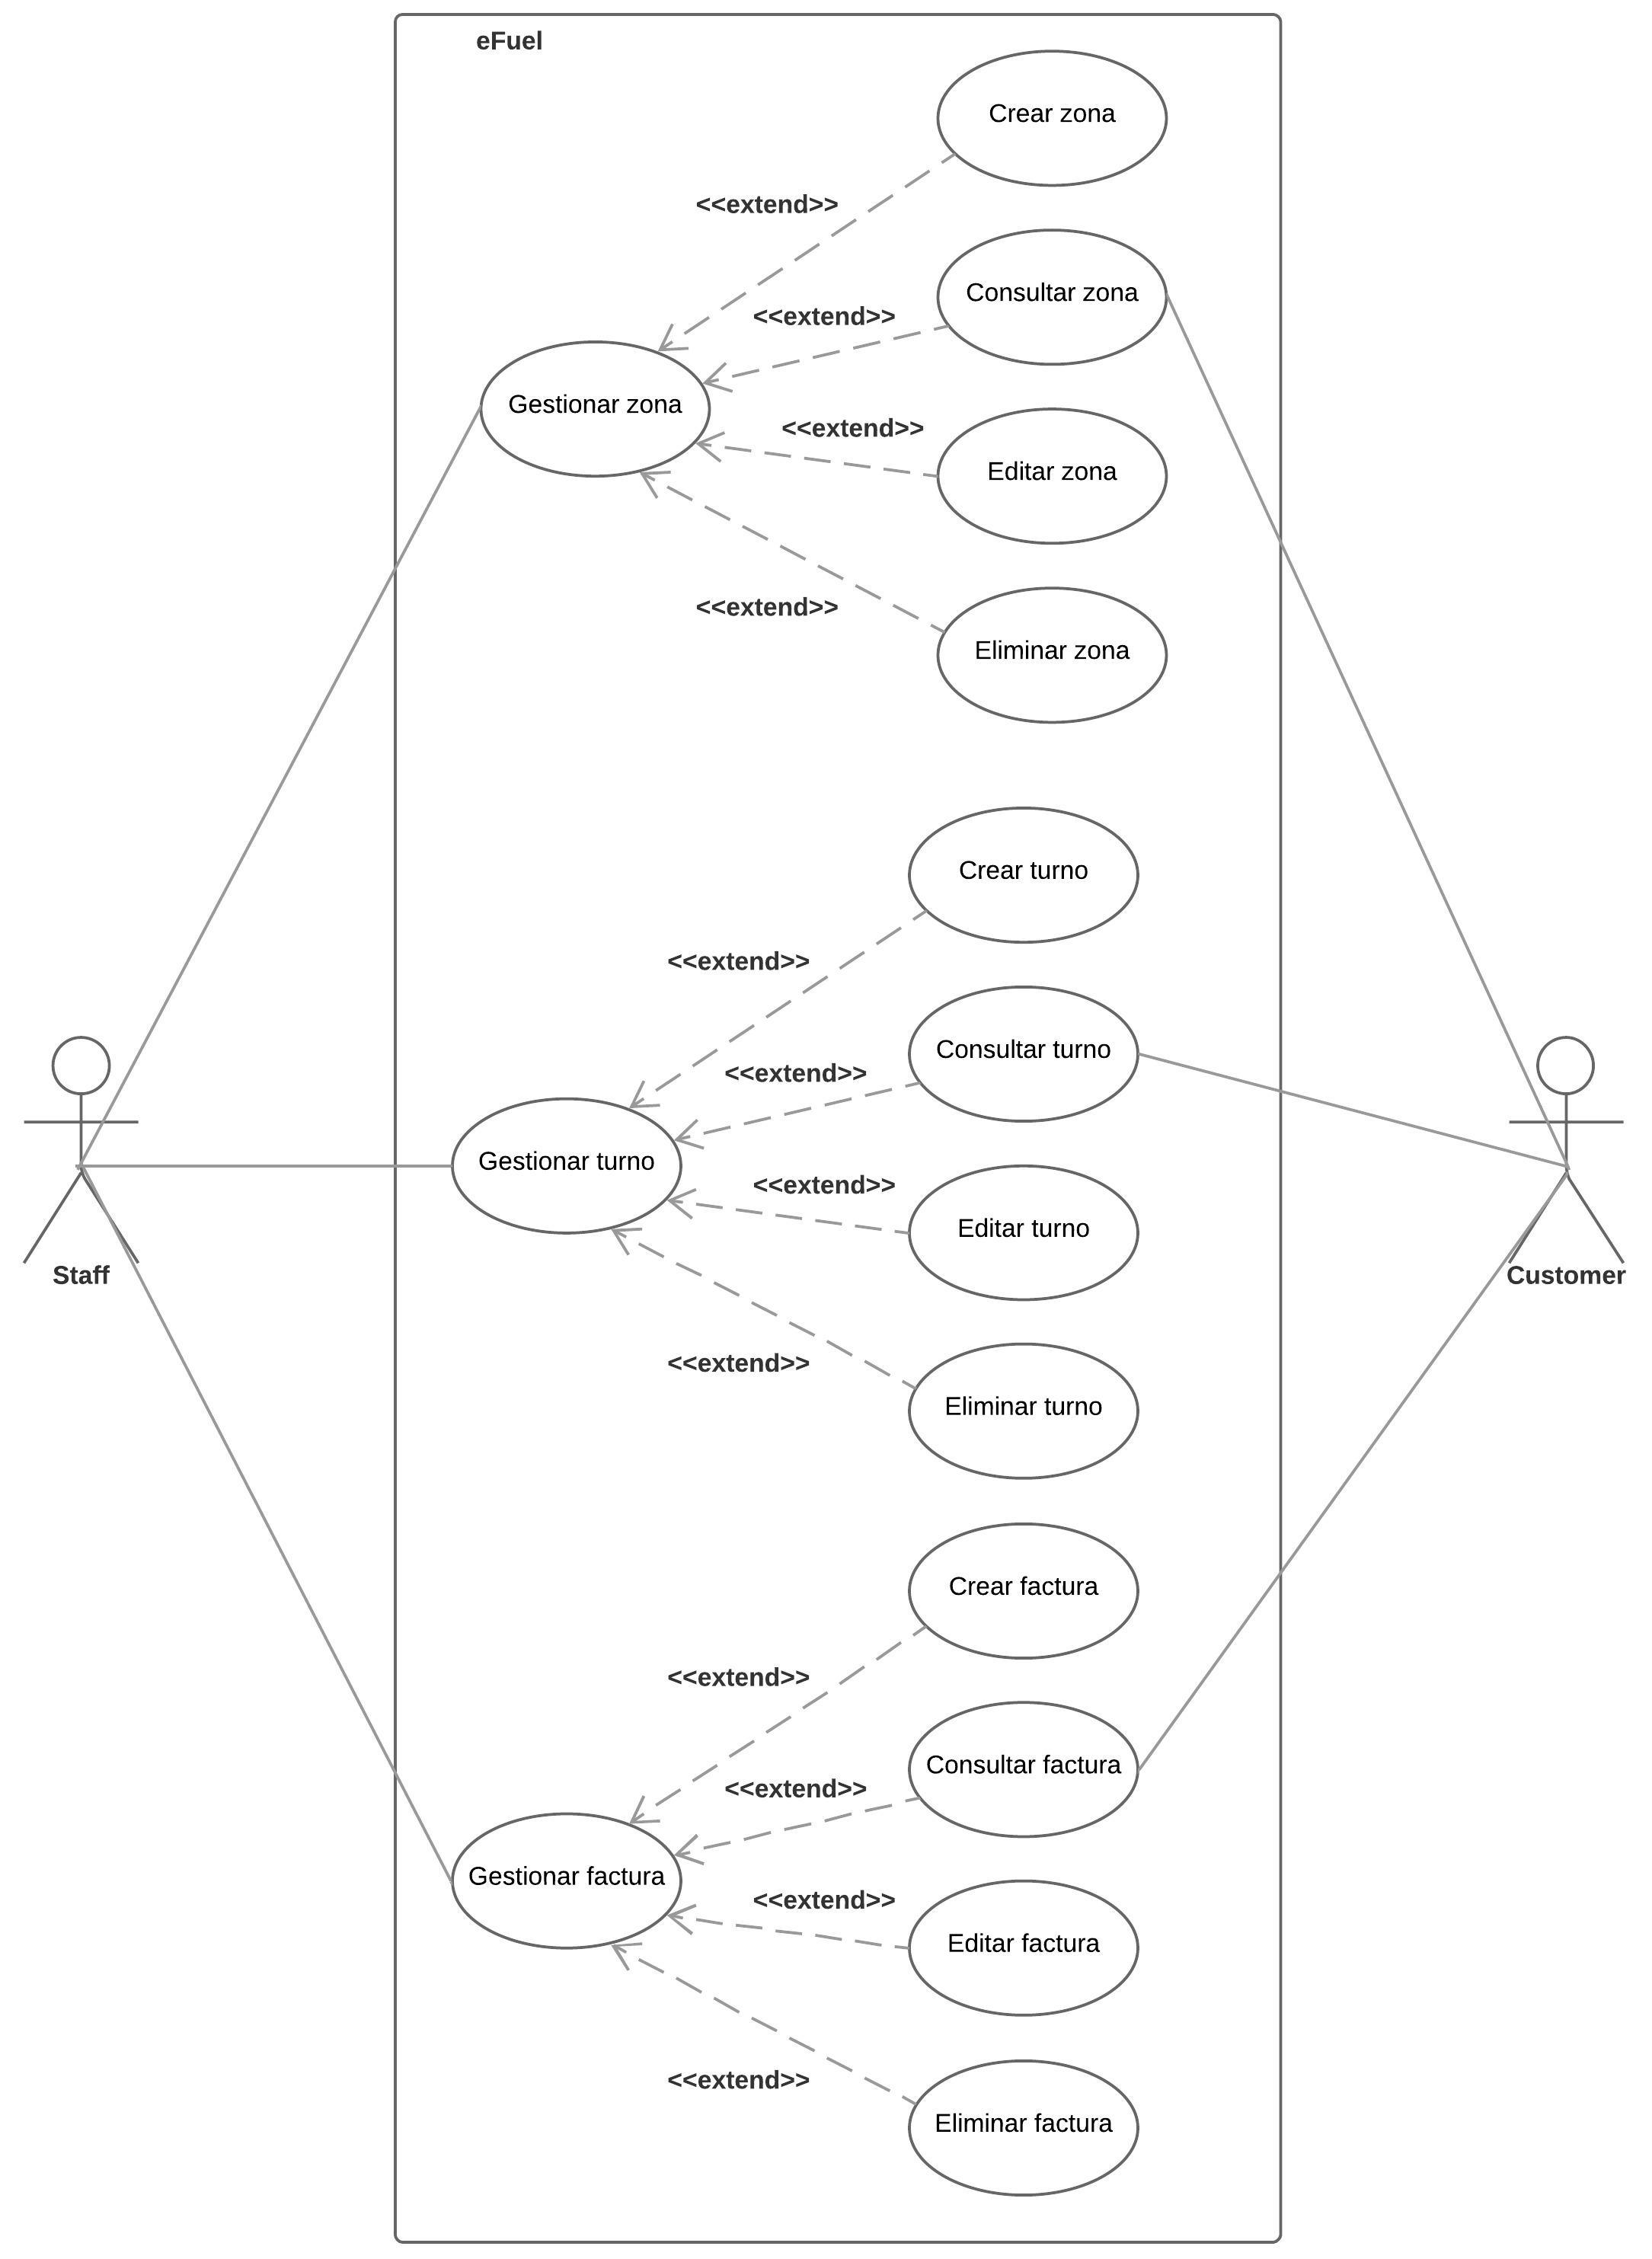
\includegraphics[width=\textwidth]{cu2.jpeg}
        \centering
    \end{figure}

    \begin{figure}[H]
        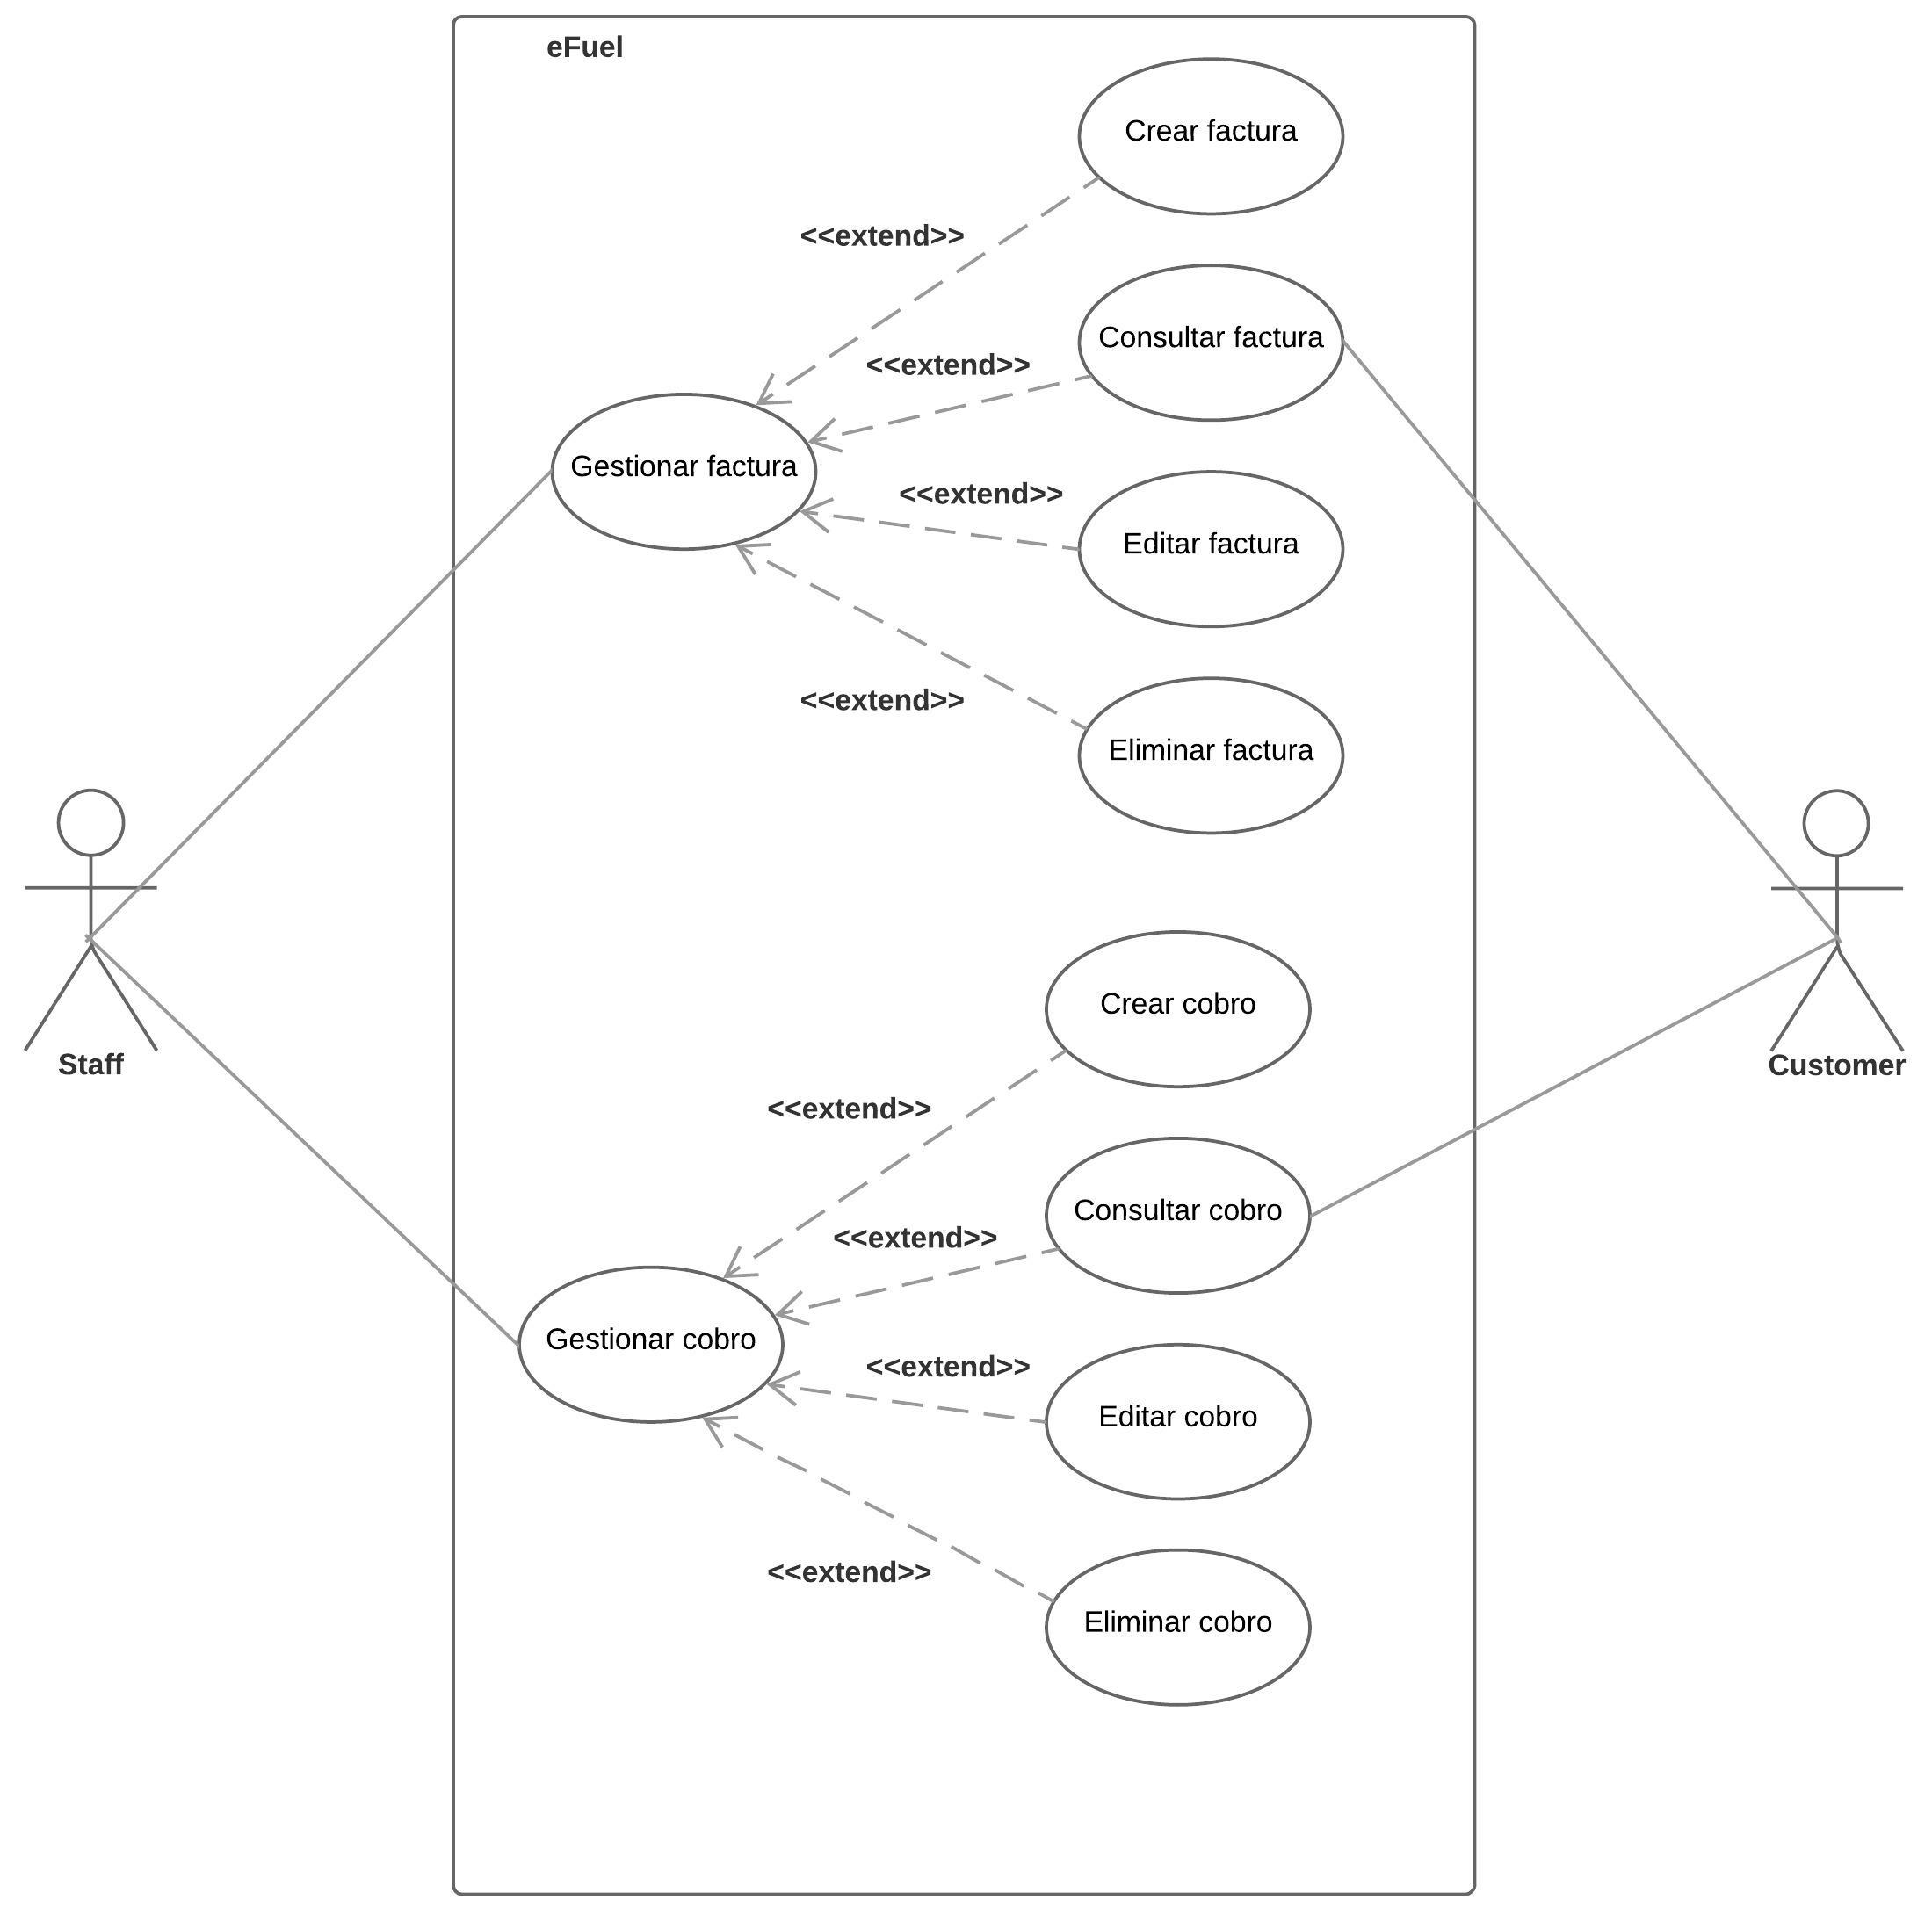
\includegraphics[width=\textwidth]{cu3.jpeg}
        \centering
    \end{figure}

    \begin{figure}[h]
        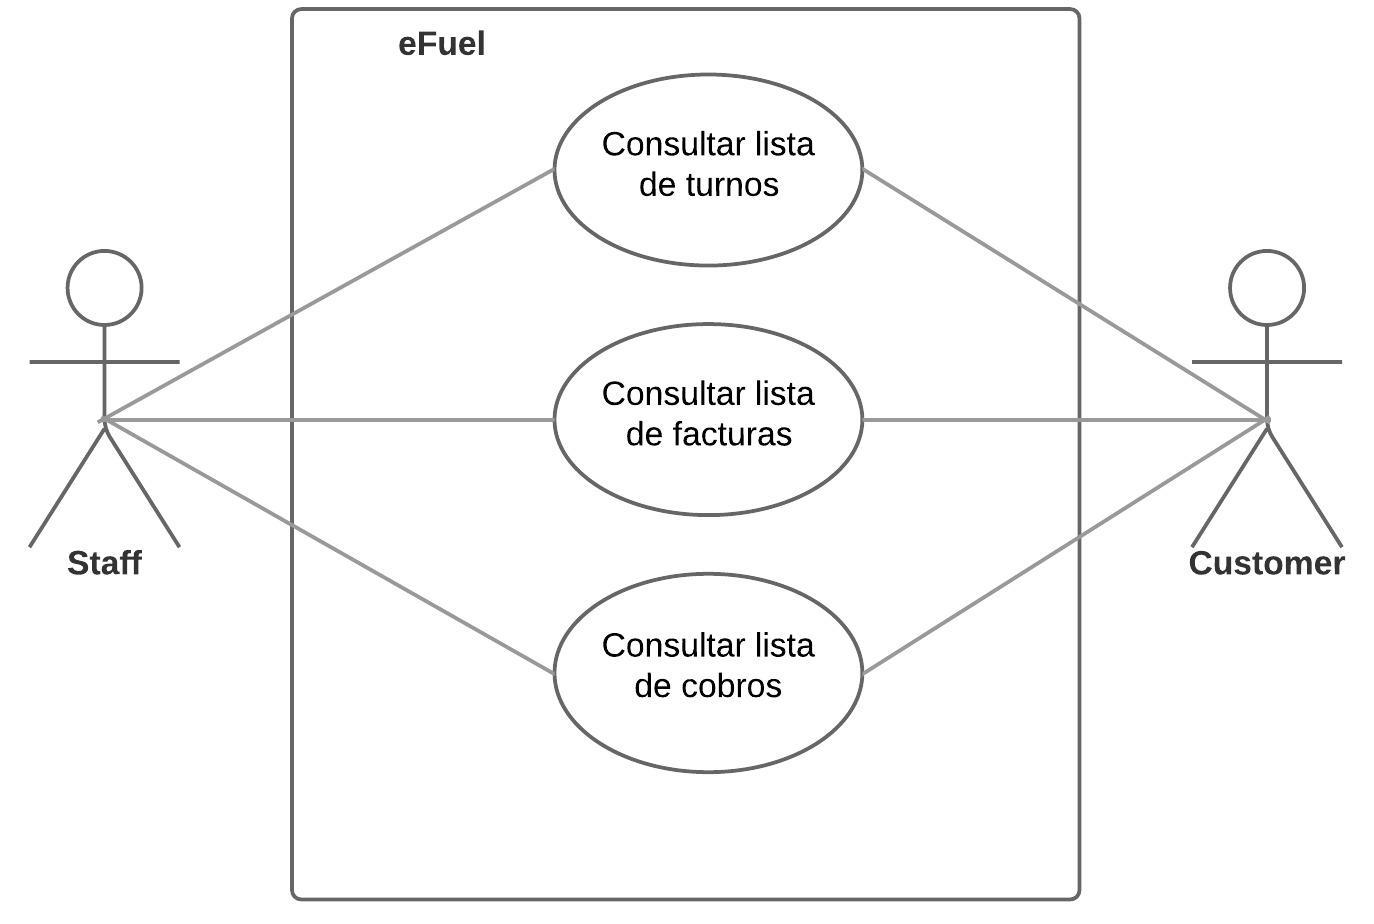
\includegraphics[width=\textwidth]{cu4.jpeg}
        \centering
    \end{figure}

    \subsection{Especificaciones de Casos de Uso}

    \section{Vista Lógica} \label{vistaLogica}
    \subsection{Vista General}
    \subsubsection{Diagrama Conceptual (Modelo de Dominio)}
    \subsubsection{Diagrama de Clases}

    \section{Vista de Implantación} \label{vistaImplantacion}
    \subsection{Configuración Estándar}
    \subsection{Diagrama de Despliegue}


    \section{Vista de Implementación} \label{vistaImplementacion}
    \subsection{Vista General}
    \subsection{Diagrama de Componentes}


    \section{Vista de Datos} \label{vistaDatos}
    \subsection{Diagrama de Entidad Relación (ER)}
    \subsection{Diccionario de Datos}


    \section{Tamaño y Desempeño} \label{tamDesemp}

    \section{Calidad}
    \subsection{Mantenibilidad}
    \subsection{Flexibilidad}
    \subsection{Seguridad}
\end{document}

